\subsubsection{Постановка задачі}
Розглядається пружне прямокутне тіло (Рис: \ref{geom_gen}), яке займає облась,
що описується у декартовій системі координат співвідношеннями $0 \le x \le a$, $0 \le y \le b$.

До грані $y=b$ додано нормальне навантаження
\begin{equation}\label{bound_1_static_1}
    \sigma_y(x, y) |_{y=b} = -p(x), \quad  \tau_{xy}(x,y) |_{y=b} =0,
\end{equation}
де $p(x)$ є відома функція.

На бічних та нижній гранях виконуються умови ідеального контакту
\begin{equation}\label{bound_2_static_1}
    u(x,y) |_{x=0} = 0, \quad \tau_{xy}(x,y) |_{x=0} =0
\end{equation}
\begin{equation}\label{bound_3_static_1}
    u(x,y) |_{x=a} = 0, \quad \tau_{xy}(x,y) |_{x=a} =0
\end{equation}
\begin{equation}\label{bound_4_static_1}
    v(x,y) |_{y=0} = 0, \quad \tau_{xy}(x,y) |_{y=0} =0
\end{equation}
Потрібно відшукати розв'язок рівняннь рівноваги
\begin{equation}\label{lame_static_1}
    \begin{cases}
        \frac{\partial^2 u(x,y)}{\partial x^2} + \frac{\partial^2 u(x,y)}{\partial y^2} + \mu_0 (\frac{\partial^2 u(x,y)}{\partial x^2} + \frac{\partial^2 v(x,y)}{\partial x\partial y}) = 0 \\
        \frac{\partial^2 v(x,y)}{\partial x^2} + \frac{\partial^2 v(x,y)}{\partial y^2} + \mu_0 (\frac{\partial^2 u(x,y)}{\partial x \partial y} + \frac{\partial^2 v(x,y)}{\partial y^2}) = 0 \\
    \end{cases}
\end{equation}
за умови виконання \eqref{bound_1_static_1} - \eqref{bound_4_static_1}.

\subsubsection{Побудова точного розв'язку вихідної задачі}
Для того, щоби звести задачу до одновимірної задачі, використано інтегральне перетворення Фур'є за змінною $x$ безпосередньо до рівнянь \eqref{lame_static_1} у наступному вигляді:
\begin{equation}
    \begin{pmatrix}
        u_n(y) \\
        v_n(y)
    \end{pmatrix} = \int_{0}^{a} 
    \begin{pmatrix}
        u(x,y) sin(\alpha_n x) \\
        v(x,y) cos(\alpha_n x)
    \end{pmatrix} dx, \quad \alpha_n = \frac{\pi n}{a}
\end{equation}

Після інтегрування обох рівнянь за частинами у просторі трансформант отримано
\begin{equation}\label{transf_static_1}
    \begin{cases}
        u_n^{''}(y) - \alpha_n \mu_0 v_n^{'}(y) - \alpha_n^2 (1 + \mu_0) u_n(y) = 0 \\
        (1 + \mu_0) v_n^{''}(y) + \alpha_n \mu_0 u_n^{'}(y)  - \alpha_n^2 v_n(y) = 0 \\
    \end{cases}
\end{equation}

Крайові умови у просторі трансформант записано у поданні
\begin{equation}\label{transf_bound_static_1}
    \begin{cases}
        \left( (2G + \lambda)v_n^{'}(y) + \alpha_n \lambda u_n(y) \right)|_{y=b} = -p_n, \\
        \left(u_n^{'}(y) - \alpha_n v_n(y)  \right)|_{y=b} = 0, \\
        v_n(y)|_{y=0} = 0, \\
        \left(u_n^{'}(y) - \alpha_n v_n(y)  \right)|_{y=0} = 0,
    \end{cases}
\end{equation}
де $p_n = \int_{0}^{a} p(x) cos(\alpha_n x) dx$.

Для того, щоби розв'язати задачу у простосторі трансформант, її переписано у векторній формі.
Рівняння рівноваги \eqref{transf_static_1} запишемо у наступному вигляді:
\begin{equation}\label{transf_mat_static_1}
    L_2\left[ Z_n(y) \right] = 0,
\end{equation}
\begin{equation}
    L_2\left[ Z_n(y) \right] = A * Z_n^{''}(y) + B * Z_n^{'}(y) + C * Z_n(y),
\end{equation}
де
\begin{equation*}
    A = \begin{pmatrix}
        1 & 0 \\
        0 & 1 + \mu_0
    \end{pmatrix}, \quad
    B = \begin{pmatrix}
        0 & -\alpha_n \mu_0 \\
        \alpha_n \mu_0 & 0
    \end{pmatrix}, \quad
    C = \begin{pmatrix}
        -\alpha_n^2(1 + \mu_0) & 0 \\
        0 & -\alpha_n^2
    \end{pmatrix}
\end{equation*}
\begin{equation*}
    Z_n(y) = \begin{pmatrix}
        u_n(y) \\
        v_n(y)
    \end{pmatrix}
\end{equation*}
Граничні умови (\ref{transf_bound_static_1}) буде зображено як
\begin{equation}\label{transf_bound_mat_static_1}
    U_i\left[ Z_n(y) \right] = D_i,
\end{equation}
\begin{equation}
    U_i\left[ Z_n(y) \right] = E_i * Z_n^{'}(b_i) + F_i * Z_n(b_i),
\end{equation}
де $i = \overline{0, 1}$, $b_0 = b$, $b_1 = 0$,
\begin{equation*}
    E_0 = \begin{pmatrix}
        1 & 0 \\
        0 & 2G + \lambda
    \end{pmatrix}, \quad
    F_0 = \begin{pmatrix}
        0 & -\alpha_n \\
        \alpha_n \lambda & 0
    \end{pmatrix}, \quad
\end{equation*}
\begin{equation*}
    E_1 = \begin{pmatrix}
        1 & 0 \\
        0 & 0
    \end{pmatrix}, \quad
    F_1 = \begin{pmatrix}
        0 & -\alpha_n \\
        0 & 1
    \end{pmatrix}, \quad
\end{equation*}
\begin{equation*}
    D_0 = \begin{pmatrix}
        0 \\
        -p_n
    \end{pmatrix}, \quad
    D_1 = \begin{pmatrix}
        0 \\
        0
    \end{pmatrix}, \quad
\end{equation*}

Потрібно відшукати розв'язок однорідного векторного рівняння \eqref{transf_mat_static_1}.
З цією метою спочатку розшукуємо розв'язок однорідного матричного рівняння.
Його побудовано у вигляді \cite{gantmaher}:
\begin{equation}
    Y(y) = \frac{1}{2\pi i} \oint_C e^{sy} M^{-1}(s)ds,
\end{equation}
де $M(s)$ - характеристична матриця рівняння \eqref{transf_mat_static_1}, $C$ - замкнений контур, який містить усі особливі точки підінтегральної функції.
Матриця $M(s)$ визначається з співвідношення
\begin{equation}
    L_2\left[ e^{sy}*I \right] = e^{sy} * M(s), \quad I = \begin{pmatrix} 1 & 0 \\ 0 & 1 \end{pmatrix},
\end{equation}
де матриця $M(s)$ має вигляд:
\begin{equation}
    M(s) = \begin{pmatrix}
        s^2 -\alpha_n^2(1 + \mu_0) & -\alpha_n \mu_0 s \\
        \alpha_n \mu_0 s & s^2 (1 + \mu_0) -\alpha_n^2
     \end{pmatrix}
\end{equation}

Матрицю $M^{-1}(s)$ побудовано у наступному поданні $M^{-1}(s) = \frac{\widetilde{M(s)}}{det[M(s)]}$, де $\widetilde{M(s)}$ - транспонована матриця алгебричних доповнень
\begin{equation}
    \widetilde{M(s)} = \begin{pmatrix}
        s^2 (1 + \mu_0) -\alpha_n^2 & \alpha_n \mu_0 s \\
        -\alpha_n \mu_0 s & s^2 -\alpha_n^2(1 + \mu_0)
     \end{pmatrix}
\end{equation}
$det[M(s)]$ - детермінант матриці
\begin{align}
    &det[M(s)] = \begin{vmatrix}
        s^2 - \alpha_n^2 - \alpha_n^2\mu_0 & -\alpha_n \mu_0 s \\
        \alpha_n \mu_0 s & s^2 (1 + \mu_0) -\alpha_n^2
     \end{vmatrix} = \nonumber \\
    &=(1+\mu_0)(s - \alpha_n)^2(s + \alpha_n)^2,
\end{align}
Детермінант матриці $det[M(s)]$ прирівнено до нуля
та встановлено його корені $\alpha_n$, та $-\alpha_n$, що є коренями другої кратності детермінанта матриці $M(s)$.
Детальне знаходження їх наведено у Додатку B.

За допомогою теореми про лишки знайдено фундаментальну матричну систему
\begin{align*}
    &\frac{1}{2\pi i} \oint_C e^{sy} M^{-1}(s)ds = \frac{2 \pi i}{2 \pi i (1 + \mu_0)} \sum_{i=1}^{2} Res\left[ e^{sy} \frac{\widetilde{M(s)}}{det[M(s)]} \right] = \\
    & = \frac{1}{(1 + \mu_0)} \left(Y_0(y) + Y_1(y) \right),
\end{align*}
де
\begin{align}\label{fund_mat_0_static_1}
    &Y_0(y) =  \frac{\partial}{\partial s} \left( \frac{e^{sy}}{(s+\alpha_n)^2} \widetilde{M(s)} \right) \Big|_{s=\alpha_n} = \nonumber \\
    &=\frac{e^{\alpha_n y}}{4\alpha_n} \begin{pmatrix}
    \alpha_n \mu_0 y + 2 + \mu_0 & \alpha_n \mu_0 y \\
    -\alpha_n \mu_0 y & -\alpha_n \mu_0 y + 2 + \mu_0
    \end{pmatrix},
\end{align}
\begin{align}\label{fund_mat_1_static_1}
    &Y_1(y) = \frac{\partial}{\partial s} \left(\frac{e^{sy}}{(s-\alpha_n)^2} \widetilde{M(s)} \right) \Big|_{s=-\alpha_n} = \nonumber \\
    =&\frac{e^{-\alpha_n y}}{4\alpha_n} \begin{pmatrix}
    \alpha_n \mu_0 y - 2 - \mu_0 & -\alpha_n \mu_0 y \\
    \alpha_n \mu_0 y & -\alpha_n \mu_0 y - 2 - \mu_0
    \end{pmatrix}
\end{align}

Розв'зок однорідного рівняння у просторі трансформант подано формулою
\begin{equation}
    Z_n(y) = \frac{1}{1 + \mu_0} \left( Y_0(y) * \begin{pmatrix} c_1 \\ c_2 \end{pmatrix} +  Y_1(y) * \begin{pmatrix} c_3 \\ c_4 \end{pmatrix}  \right),
\end{equation}
де $c_i$, $i=\overline{1, 4}$ - невідомі константи, щоби їх відшукати використано граничні умови \eqref{transf_bound_mat_static_1} (\nameref{ap_E}).

Таким чином, отримано розв'язок векторної крайової задачі у просторі трансформант Фур'є:
\begin{align}\label{transf_sol_u_static_1}
    &u_n(y) = \frac{e^{\alpha_n y}}{4 \alpha_n (1 + \mu_0)} \left[c_1 (\alpha_n \mu_0 y + 2 + \mu_0) + c_2 (\alpha_n \mu_0 y) \right] + \nonumber \\
    &\quad + \frac{e^{-\alpha_n y}}{4 \alpha_n (1 + \mu_0)} \left[c_3 (\alpha_n \mu_0 y - 2 - \mu_0) + c_4 (-\alpha_n \mu_0 y)\right]
\end{align}
\begin{align}\label{transf_sol_v_static_1}
    &v_n(y) = \frac{e^{\alpha_n y}}{4 \alpha_n (1 + \mu_0)} \left[c_1 (-\alpha_n \mu_0 y) + c_2 (-\alpha_n \mu_0 y + 2 + \mu_0) \right] + \nonumber \\
    &\quad + \frac{e^{-\alpha_n y}}{4 \alpha_n (1 + \mu_0)} \left[c_3 (\alpha_n \mu_0 y) + c_4 (-\alpha_n \mu_0 y - 2 - \mu_0)\right]
\end{align}

Для того, щоб виписати подання для поля переміщень вихідної задачі обернене перетворення Фур'є застосовано до формул \eqref{transf_sol_u_static_1}, \eqref{transf_sol_v_static_1}
\begin{equation}
    u(x,y) = \frac{2}{a} \sum_{n=1}^{\infty} u_n(y) sin(\alpha_n x), \quad \alpha_n = \frac{\pi n}{a}
\end{equation}
\begin{equation}
    v(x,y) = \frac{v_0(y)}{a} + \frac{2}{a} \sum_{n=1}^{\infty} v_n(y) cos(\alpha_n x), \quad \alpha_n = \frac{\pi n}{a}
\end{equation}

Останній крок - це знаходження виразу $v_0(y)$ у випадку коли $n=0$, $\alpha_0 =0$.
Для цього випадку рівняння для його визначення записано у формі
\begin{equation}\label{transf_v_0_static_1}
    (1 + \mu_0) v_0^{''}(y) = 0
\end{equation}
Граничні умови набувають вигляду
\begin{equation}\label{transf_bound_v_0_static_1}
    \begin{cases}
        (2G + \lambda)v_0^{'}(y)|_{y=b} = -p_0, \\
        v_0(y)|_{y=0} = 0,
    \end{cases}
\end{equation}
де $p_0 = \int_{0}^{a}p(x)dx$.

Невідомі константи загального розв'язку $v_0(y) = c_1 + c_2 y$ визначено з умов \eqref{transf_bound_v_0_static_1}.

Отже 
\begin{equation}
    v_0(y) = \frac{-p_0}{(2G + \lambda)}y
\end{equation}
З цього випливає остаточне подання розв'язку вихідної задачі
\begin{equation}
    \begin{cases}
        u(x,y) = \frac{2}{a} \sum_{n=1}^{\infty} u_n(y) sin(\alpha_n x), \quad \alpha_n = \frac{\pi n}{a} \\
        v(x,y) = \frac{-p_0}{(2G + \lambda)a}y + \frac{2}{a} \sum_{n=1}^{\infty} v_n(y) cos(\alpha_n x), \quad \alpha_n = \frac{\pi n}{a}
    \end{cases}
\end{equation}

\subsubsection{Числові розрахунки та обговорення}
Числові експеременти наведено для сталі ($E=200$ ГПА, $\mu=0.25$).

Розглянуто прямокунту область $0 \le x \le 10$, $0 \le y \le 15$, функцію навантаження взято у формі $p(x)=(x-2.5)^2$.
На рисунках (Рис: \ref{static_1_u_1}) - (Рис: \ref{static_1_sigma_y_1})
представлено функції переміщень $u(x,y)$, $v(x,y)$ та напружень $\sigma_x(x,y)$, $\sigma_y(x,y)$ відповідно.
\begin{figure}[h!]
    \begin{center}
        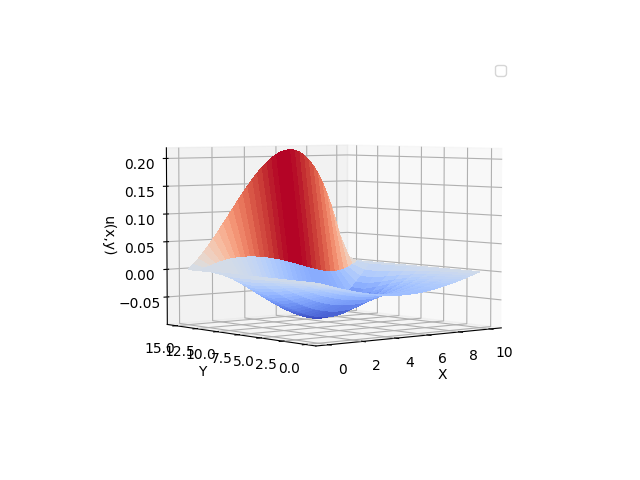
\includegraphics[width=0.49\textwidth, scale=1]{images/results/static_1/function_u_1.png}
        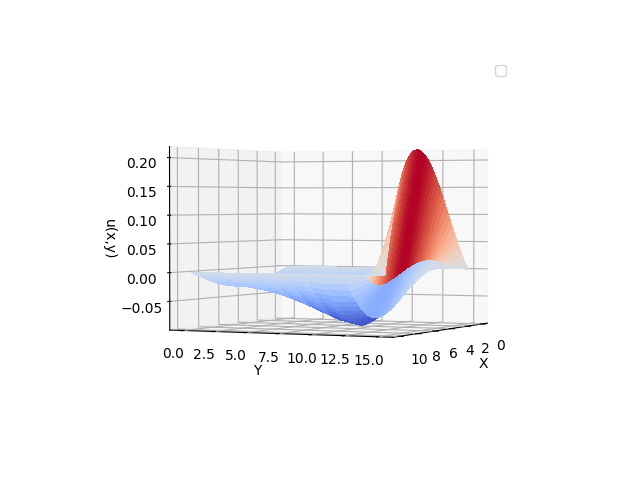
\includegraphics[width=0.49\textwidth, scale=1]{images/results/static_1/function_u_2.png}
        \caption{Функція $u(x, y)$}\label{static_1_u_1}
    \end{center}
\end{figure}
\newpage
\begin{figure}[h!]
    \begin{center}
        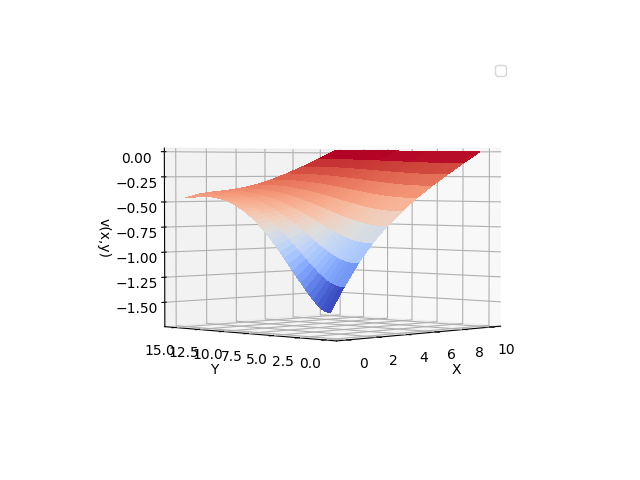
\includegraphics[width=0.49\textwidth, scale=1]{images/results/static_1/function_v_1.png}
        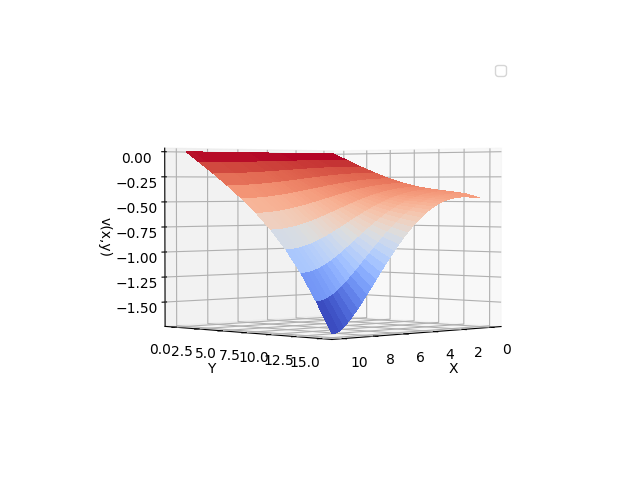
\includegraphics[width=0.49\textwidth, scale=1]{images/results/static_1/function_v_2.png}
        \caption{Функція $v(x, y)$}\label{static_1_v_1}
    \end{center}
\end{figure}
\begin{figure}[h!]
    \begin{center}
        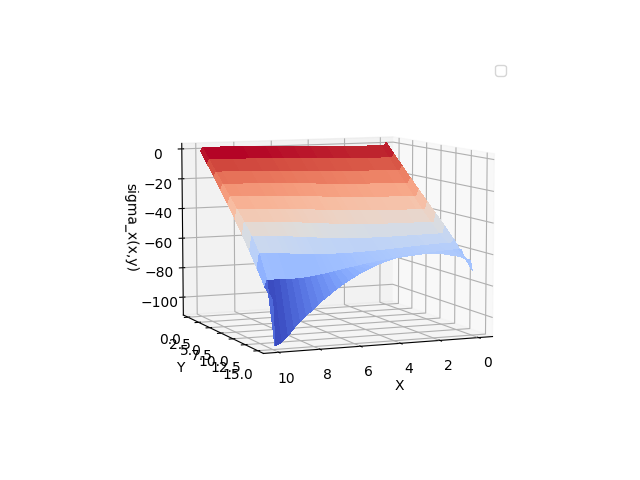
\includegraphics[width=0.49\textwidth, scale=1]{images/results/static_1/function_sigma_x_1.png}
        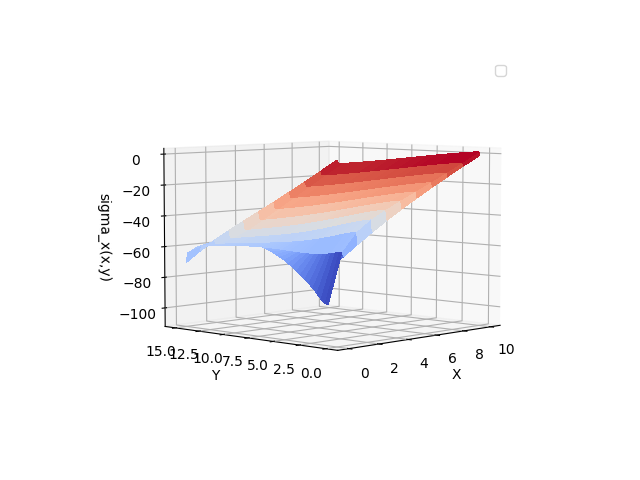
\includegraphics[width=0.49\textwidth, scale=1]{images/results/static_1/function_sigma_x_2.png}
        \caption{Функція $\sigma_x(x, y)$}\label{static_1_sigma_x_1}
    \end{center}
\end{figure}
\begin{figure}[h!]
    \begin{center}
        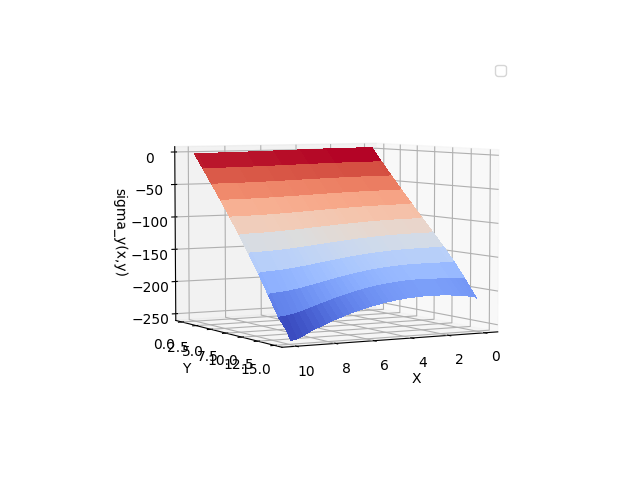
\includegraphics[width=0.49\textwidth, scale=1]{images/results/static_1/function_sigma_y_1.png}
        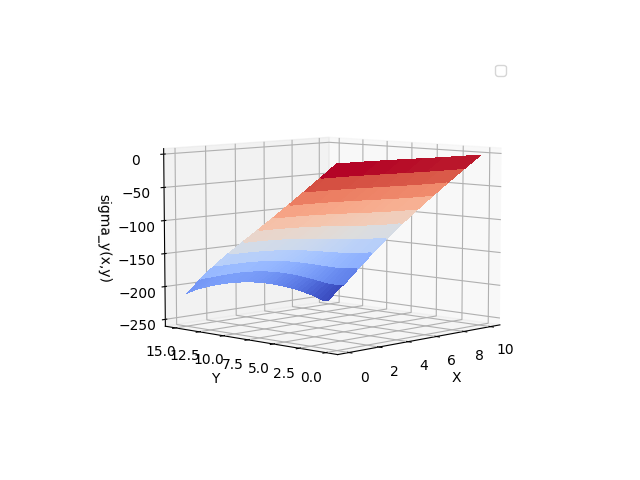
\includegraphics[width=0.49\textwidth, scale=1]{images/results/static_1/function_sigma_y_2.png}
        \caption{Функція $\sigma_y(x, y)$}\label{static_1_sigma_y_1}
    \end{center}
\end{figure}
